\scanpage{28}

It is thus a group scheme over $S_0=\operatorname{Spec}\mathbb{Z}$
all of whose fibers are reduced to the trivial
group, except for the \unsure{generic} fiber, which is
$ {\mathbb{G}_a^{\,n}}_{\mathbb{Q}}$.

\deleted{\unsure{And}}
In the case of an arbitrary metabelian
group $\mathcal{G}$, \unsure{denoting|let us denote} by
$\widehat{\mathcal{G}}$ its
profinite \unsure{completion}, by $\widehat{\mathcal{G}}_{S_0}$ the
profinite group scheme over $\unsure{S_0}$.
\[
(50)\qquad
\widehat{\mathcal{G}}_{S_0}
\overset{\mathrm{dfn}}{=}\varprojlim_i(H_i)_{S_0}
\]
we shall \unsure{thereby} have a canonical exact sequence
\[
(51)\qquad
\diagram{\begin{tikzcd}[column sep=large]
1 \arrow[r] &
\operatorname{Env}^{0}(\mathcal{G})
\arrow[r,very thick,"\deleted{\unsure{\mathrm{dfn}}}"] &
\varprojlim\operatorname{Env}(\mathcal{G}) \arrow[r] &
(\widehat{\mathcal{G}})_{S_0} \arrow[r] & 1
\end{tikzcd}}
\]
where $\operatorname{Env}^{0}(\mathcal{G})$ denotes the identity component
of $\unsure{\varprojlim}\operatorname{Env}(\mathcal{G})$, i.e.
\[
\begin{aligned}
(52)\qquad
\operatorname{Env}^{0}(\mathcal{G})
&\overset{\mathrm{dfn}}{=}\varprojlim_i\underline{M}_i\\
&\simeq\varprojlim_n n.\,\underline{M}_0
\end{aligned}
\]
where the $M_i$ are the subgroups of finite
index in $\mathcal{G}$ \deleted{\unsure{such that|such that}}
which are free $\mathbb{Z}$-modules of finite type, where
(as above) for such a $\mathbb{Z}$-module $M$,

\figure{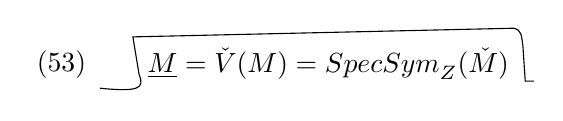
\begin{tikzpicture}[baseline=(eq.base)]
\node[anchor=base west,inner sep=0pt] (eq) at (0,0)
{$\underline{M}=\check{V}(M)=\operatorname{Spec}\operatorname{Sym}_{\mathbb{Z}}(\check{M})$};
\node[anchor=east] at ([xshift=-0.65cm]eq.west) {$(53)$};
\draw
([xshift=-0.60cm,yshift=-0.10cm]eq.south west)
.. controls ([xshift=-0.10cm,yshift=-0.15cm]eq.south west)
and ([xshift=-0.03cm,yshift=-0.10cm]eq.south west)
.. ([xshift=-0.10cm,yshift=0.07cm]eq.south west)
-- ([xshift=-0.18cm,yshift=0.14cm]eq.north west)
-- ([xshift=0.05cm,yshift=0.25cm]eq.north east)
.. controls ([xshift=0.16cm,yshift=0.23cm]eq.north east)
and ([xshift=0.15cm,yshift=0.15cm]eq.north east)
.. ([xshift=0.17cm,yshift=0.03cm]eq.north east)
-- ([xshift=0.20cm,yshift=-0.01cm]eq.south east)
-- ([xshift=0.31cm,yshift=-0.01cm]eq.south east);
\end{tikzpicture}}
denotes the vector bundle \unsure{covariant|canonical} in $M$ which it defines, and

\margin{27}

\scanpage{29}
\mspage{662}

where $M_0$ is one of the $M_i$, giving rise
to the system (cofinal in that of all the
$M_i$) of the $nM_0$. The choice of a
basis of $M_0$ over $\mathbb{Z}$ gives an
isomorphism
\[
(54)\qquad
\begin{aligned}
\operatorname{Env}^{0}(\mathcal{G})
&\simeq \operatorname{Env}^{0}(M_0)
\simeq \bigl(\operatorname{Env}^{0}(\mathbb{Z})^{\unsure{0}}\bigr)^n\\
&\simeq(\mathcal{E}^{1})^n
\end{aligned}
\]

\margin{$\unsure{\dagger}$ where
\diagram{\begin{tikzcd}[column sep=large]
(\mathbb{E}^{1},\unsure{mn|nm}) \arrow[r] &
(\mathbb{E}^{1},\uuline{n})
\end{tikzcd}}
is multiplication by $m$}

\[
(55)\qquad
\begin{aligned}
\mathcal{E}^{1}
&\simeq \operatorname{Env}^{0}(\mathbb{Z})
\simeq\operatorname{Spec}\bigl(\mathbb{Z}+T\mathbb{Q}[T]\bigr)\\
&\inserted{\simeq\varprojlim_n(\mathbb{E}^{1},n)\,\unsure{\dagger}}
\end{aligned}
\]
is the group scheme considered
above, which represents the group-valued functor
\[
(56)\qquad
A\longmapsto\mathcal{E}^{1}(A)
=\deleted{\unsure{\varprojlim}}
\left\{(x_n)\in A^{\mathbb{N}^{*}}\ \middle|\
\begin{gathered}
x_n=mx_{mn}\\[-2pt]
\forall m,n\in\unsure{\mathbb{N}^{*}}
\end{gathered}
\right\}.
\]

[If $A$ is such that there exists $n\in\mathbb{N}^{*}$ with
$nA\,\unsure{=|\simeq}\,0$ ---
\deleted{\unsure{precisely}}
which means
that the residue characteristics of $A$ divide $n$,
and \deleted{\unsure{it is}} there probably exists such an $n$
as soon as the residue characteristics of $A$ are
all $>0$ --- then $\mathcal{E}^{1}(A)=\{1\}$ ---
if on the other hand $A$ of characteristic $0$, we have $\mathcal{E}^{1}(A)\simeq A$]

\margin{28}

\scanpage{30}

5. \uline{Universal characterization} of the schematic envelope of a metabelian group.

Let $G$ be a group scheme \unsure{locally} of finite presentation over a base $S$.
We say that a \unsure{homomorphism} of group schemes
\diagram{\begin{tikzcd}
H \arrow[r] & G
\end{tikzcd}}
is \deleted{\unsure{quasi-}} \uline{unipotent} (resp. quasi-unipotent) if the image of $\forall$ \unsure{element} of $H$ is a unipotent element (resp. quasi unipotent) of $G$ --- which is checked fiber by fiber. A \unsure{homomorphism} from a discrete group
\diagram{\begin{tikzcd}
\mathcal{G} \arrow[r] & \Gamma(G/S)
\end{tikzcd}}
is said to be unipotent (resp. quasi-unipotent) if the \unsure{homomorphism} of group schemes \deleted{\unsure{associated}} \inserted{which} corresponds to it
\diagram{\begin{tikzcd}
\mathcal{G}_S \arrow[r] & G
\end{tikzcd}}
is unipotent (resp. quasi-unipotent).

\margin{29}

\scanpage{31}
\mspage{663}

Note that by the properties of $\varprojlim$ of filtered projective systems (with affine transition morphisms) \deleted{between} of schemes, if $\mathcal{G}$ is metabelian, whence a projective system of affine group schemes over $S_0$, hence over $S$, denoted $\operatorname{Env}_{\unsure{\underline{S}|S}}(\mathcal{G})$, and a projective limit
\[
\begin{aligned}
(57)\qquad L\operatorname{Env}_S(\mathcal{G})
 &=L\operatorname{Env}(\mathcal{G})\times_{S_0}S\\
 &\simeq\varprojlim\operatorname{Env}_S(\mathcal{G}),
\end{aligned}
\]
we have, as soon as $G$ is \unsure{locally} of finite presentation

(58)\quad
\diagram{\begin{tikzcd}[column sep=large,row sep=large]
\operatorname{Hom}_{\mathrm{progr}/S}(\operatorname{Env}_S(\mathcal{G}),G)
 \arrow[r,"\sim"] \arrow[d,equal,"\mathrm{def}"']
 & \operatorname{Hom}(\operatorname{Env}_S(\mathcal{G}),G)\\
\varprojlim_i\unsure{\operatorname{Hom}}(\underline{\mathcal{G}}_{i\,S},G) &
\end{tikzcd}}

Note on the other hand that we have a \deleted{\unsure{a}} canonical \unsure{homomorphism}

(59)\quad
\diagram{\begin{tikzcd}
\mathcal{G}_S \arrow[r] & \deleted{\unsure{\varprojlim}}L\operatorname{Env}_S(\mathcal{G})
\end{tikzcd}}
deduced by \unsure{change} of base from the \unsure{homomorphism} over the universal base $S_0$

(59 bis)\quad
\diagram{\begin{tikzcd}
\mathcal{G}_{S_0} \arrow[r] & L\operatorname{Env}(\mathcal{G})
\end{tikzcd}}
coming from the system of canonical \unsure{homomorphisms}

\margin{30}

\scanpage{32}

\diagram{\begin{tikzcd}
\underline{\mathcal{G}}_{S_0}\arrow[r]&\underline{\mathcal{G}}_i
\end{tikzcd}}.

Thus, via (59) we find

(60)\quad
\diagram{\begin{tikzcd}[column sep=large,row sep=large]
\operatorname{Hom}_{S\text{-}\mathrm{gr}}(L\operatorname{Env}_S(\mathcal{G}),G)
 \arrow[r] & \operatorname{Hom}_{S\text{-}\mathrm{gr}}(\mathcal{G}_S,G)
 \arrow[d,phantom,"\simeq"{rotate=90}]\\
 & \operatorname{Hom}_{\mathrm{gr}}(\mathcal{G},\Gamma(G/S))
\end{tikzcd}}

\unsure{1}

\unsure{Composing} (58) and (60), we find
\[
(61)\quad\left\{
\begin{aligned}
&\operatorname{Hom}_{\mathrm{pro}\text{-}S\text{-}\mathrm{gr}}\unsure{\ell}
 (\operatorname{Env}_S(\mathcal{G}),G)
 \simeq\operatorname{Hom}_{S\text{-}\mathrm{gr}}(L\operatorname{Env}_S(\mathcal{G}),G)\\[1.2em]
&\hspace{5em}\longrightarrow\operatorname{Hom}_{S\text{-}\mathrm{gr}}(\mathcal{G}_S,G)
 \simeq\operatorname{Hom}_{\mathrm{gr}}(\mathcal{G},G(S))
\end{aligned}\right.
\]
This being so, we have the following result

\uline{Theorem} \deleted{\unsure{If}} Under the preceding conditions

\margin{\figure{
\begin{tikzpicture}
\draw[line width=.3pt] (0,0) -- (-.015,-5.6);
\end{tikzpicture}}}
($\mathcal{G}$ a discrete metabelian group, $G$ a group scheme locally of finite presentation over a base \unsure{scheme} $S$), the canonical map (61) is \deleted{\uline{bijective} if we assume moreover, so as not to tire \unsure{myself|oneself}, that} \inserted{injective, and has as image} \unsure{the set} of \unsure{homomorphisms} \uline{quasi-unipotent} from $\mathcal{G}$ into $G(S)$ --- at least if we assume, to simplify life for ourselves, that $S$ is \unsure{noetherian} and $G$ affine over $\unsure{S|S_0}$.

\margin{31}

\scanpage{33}
\mspage{664}

\uline{5\unsure{1|0}} \uline{Example} : The Fermat ``tower''.

1. The groups $\mathcal{G},\underline{\mathcal{G}}$.

I am interested in the quotient of $\mathcal{G}_0^{\deleted{\unsure{\wedge}}}=\operatorname{GL}(2,\mathbb{Z})$ obtained by taking the quotient by $[\Pi_0,\Pi_0]$ --- we find an extension $\mathcal{G}$ of $\mathcal{G}_0/\Pi_0$ by the group

\margin{$\Pi_0$ generated by the $\lambda_i=-\ell_i$,\quad
$\displaystyle \ell_0=\begin{pmatrix}1&-2\\0&1\end{pmatrix}$\quad
$\displaystyle \ell_1=\begin{pmatrix}1&0\\2&1\end{pmatrix}$.}

\[
\begin{aligned}
(1)\qquad M\overset{\mathrm{dfn}}{=}\Pi_{0\,\mathrm{ab}}
\simeq
\Bigl(
\underset{\deleted{\underbrace{\hphantom{\mathbb{Z}(0)+\mathbb{Z}(1)+\mathbb{Z}(\infty)}}_{M}}}
{\overset{\deleted{\unsure{\wedge}}}{\mathbb{Z}}(0)+
 \overset{\deleted{\unsure{\wedge}}}{\mathbb{Z}}(1)+
 \overset{\deleted{\unsure{\wedge}}}{\mathbb{Z}}(\infty)}
\Bigr)/\text{diagonal}
\end{aligned}
\]
Thus we have an exact sequence of profinite groups

(2)\quad
\diagram{\begin{tikzcd}[column sep=large,row sep=large]
1\arrow[r] & M\arrow[r]\arrow[d,phantom,"\simeq"{rotate=90}]
 &\mathcal{G}\arrow[r]
 &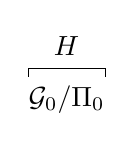
\begin{tikzpicture}[baseline=(q33.base)]
\node[inner sep=0pt] (q33) {$\mathcal{G}_0/\Pi_0$};
\draw[line width=.3pt] ([yshift=3pt]q33.north west)--([yshift=6pt]q33.north west)--([yshift=6pt]q33.north east)--([yshift=3pt]q33.north east);
\node[above=7pt] at (q33.north) {$H$};
\end{tikzpicture}\arrow[r]\arrow[d,phantom,"\simeq"{rotate=90}]
 &1\\
 &\begin{gathered}\Pi_{0\,\mathrm{ab}},\text{ also denoted}\\\mathcal{G}^{\circ}\end{gathered}
 &&\operatorname{GL}(2,\mathbb{Z}/4\mathbb{Z})/(\dot{\ell}_0,\dot{\ell}_1)&
\end{tikzcd}}

In terms of generators and relations we have
\[
(3)\quad\mathcal{G}=\left\{\tau',\rho,\sigma\;\middle|\;
\begin{aligned}
&\rho^6=\sigma^4={\tau'}^2=1\\
&\rho^3=\sigma^2,\quad\tau'(\rho)=\rho^{-1},\quad\tau'(\sigma)=\sigma^{-1}\\
&\deleted{\unsure{\rho}}[\lambda_0,\lambda_1]=1,\quad\text{where}
\end{aligned}\right.
\]
\[
\hspace{8em}\left\{
\begin{aligned}
\lambda_0&=-\ell_0=-\sigma\rho\sigma\rho=\sigma(\rho)\rho^{\deleted{\unsure{-1|4}}}\\
\lambda_1&=-\ell_1=-\rho\sigma\rho\sigma=\rho\sigma(\rho)
\end{aligned}\right.
\]
\unsure{of which|thus} the commutation relation $[\lambda_0,\lambda_1]=1$ is also written
\[
(4)\qquad \sigma(\rho)\rho^2\sigma(\rho)=\rho\sigma(\rho^2)\rho
\qquad\text{or again}
\]
\[
(5)\qquad -\sigma\underbrace{\rho\sigma\rho^{-1}\sigma\rho}\sigma
=\underbrace{\rho\sigma\rho^{-1}\sigma\rho}
\]
where the play of the $-$ signs can be made explicit in the formalism of generators and relations by removing this sign from the formula, and replacing in \unsure{return} one (or an odd \unsure{num\textsuperscript{b}er|number}) of the $\sigma$ in the formula by $\sigma^{-1}$. For example, the formula

\margin{32}